\section{Results}
\label{sec:results}

\subsection{Diminishing returns from case volume for the mean reproduction number}
\label{sec:res-theory}

\begin{figure}[t]
  \centering
  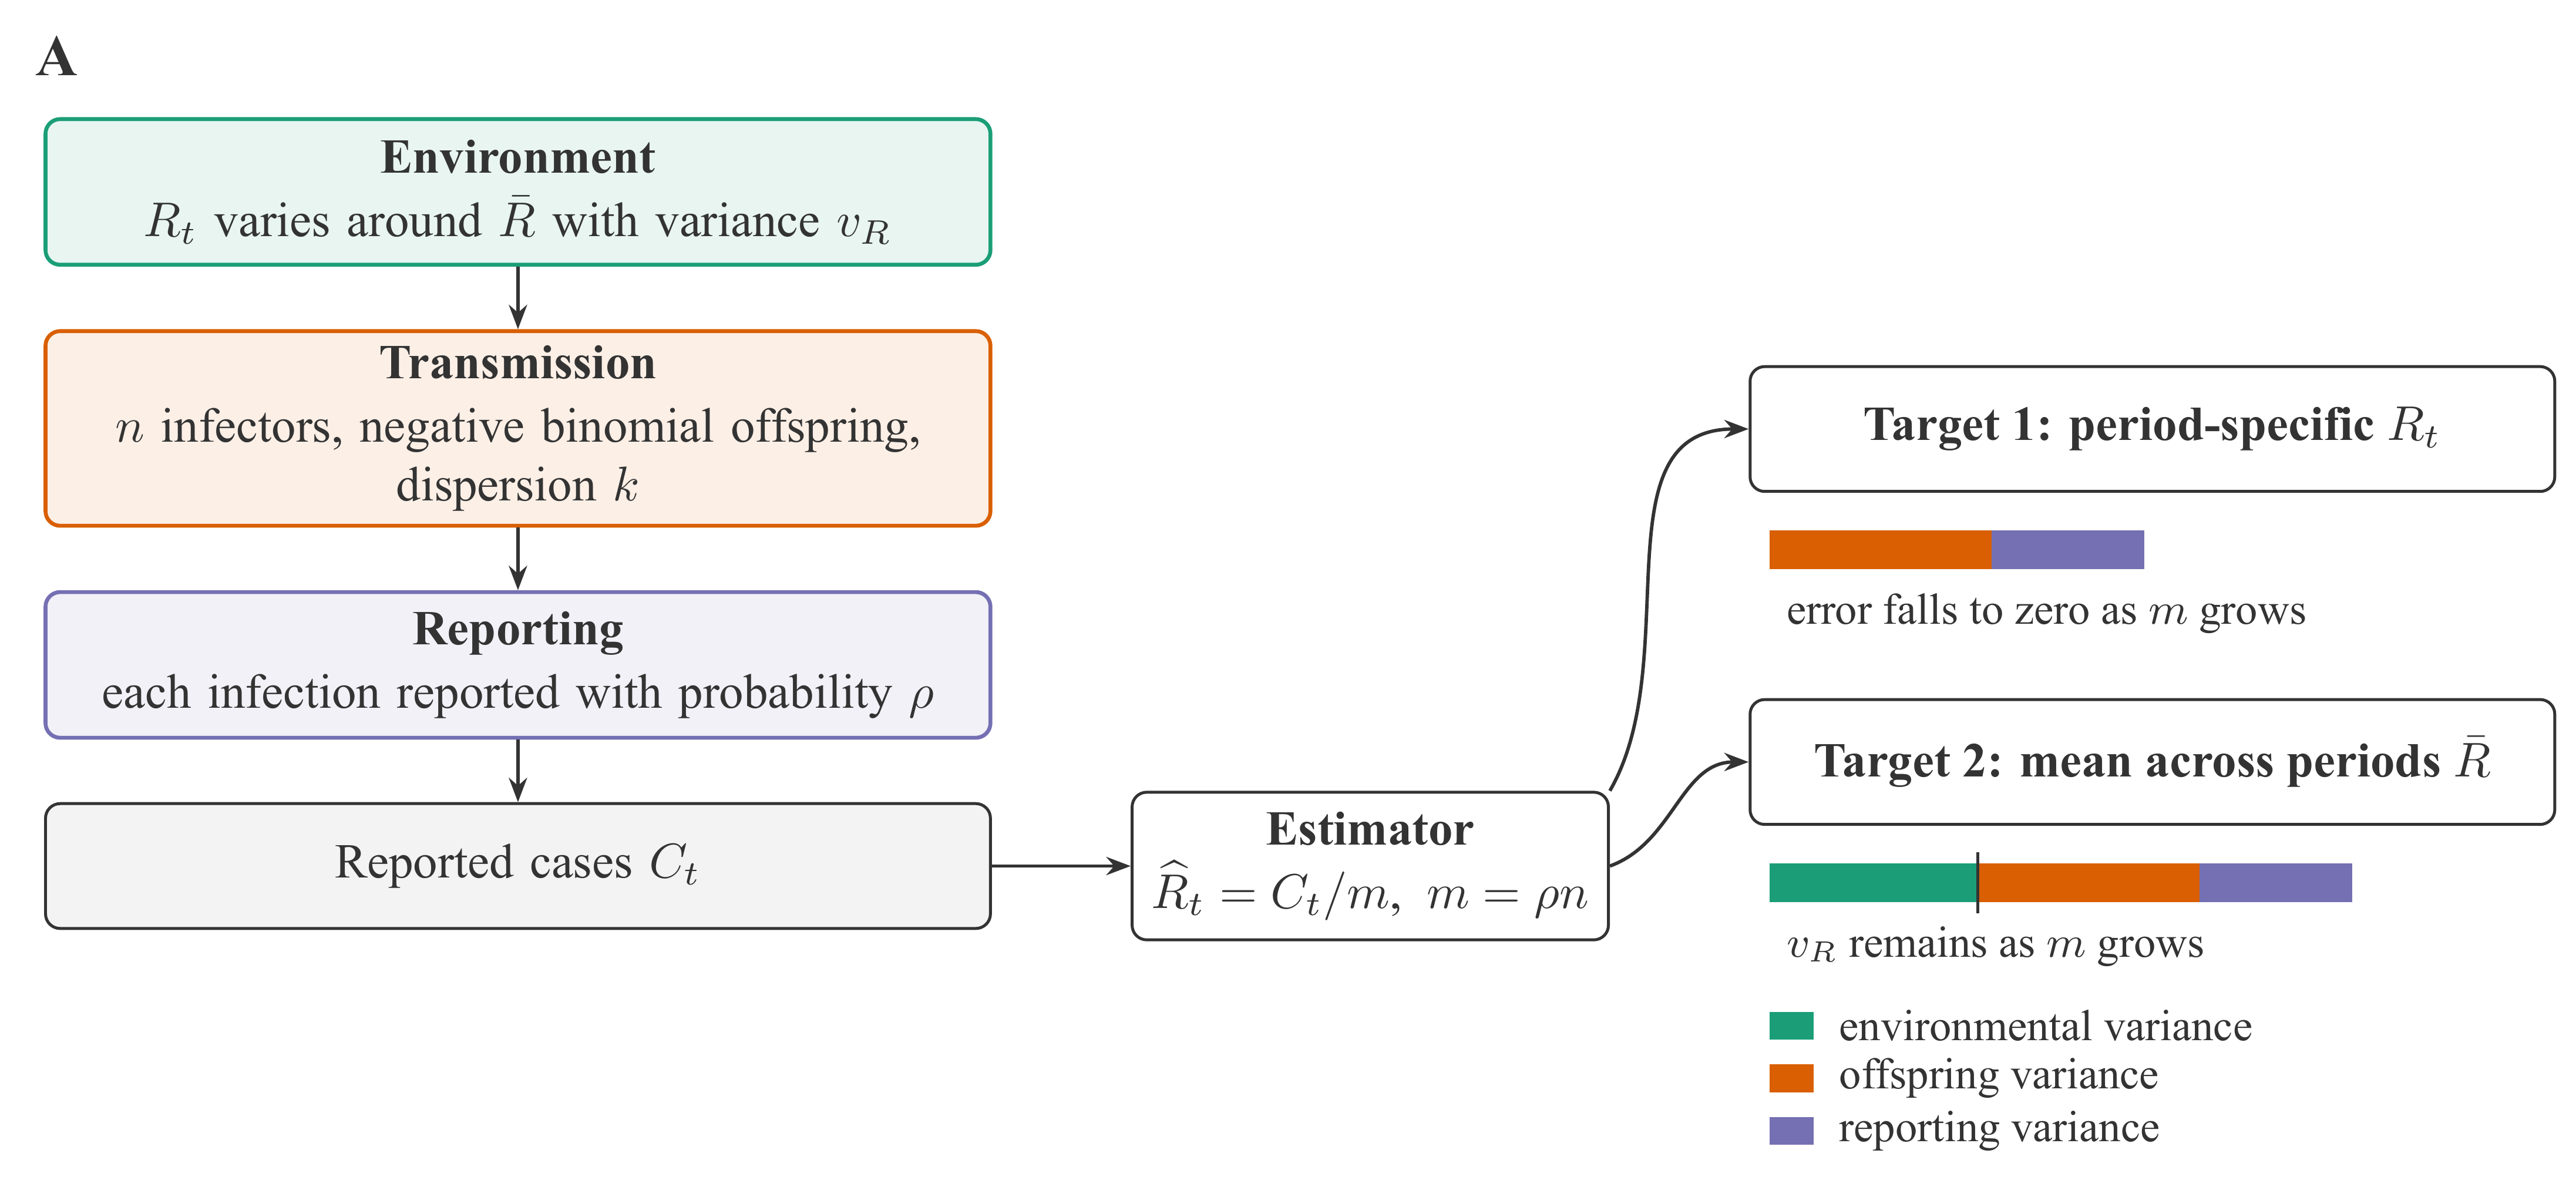
\includegraphics[width=0.86\linewidth]{figures/fig_01_schematic.png}\\[2pt]
  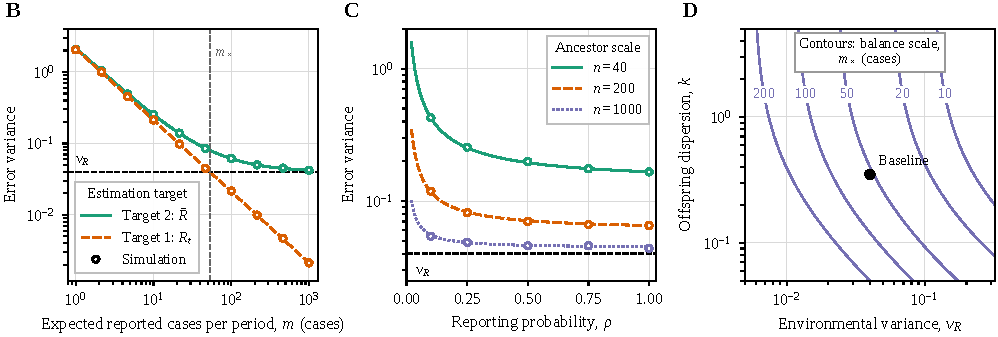
\includegraphics[width=\linewidth]{figures/fig_01_theory.pdf}
  \caption{Contributions of environmental, offspring and reporting variation to the error of the scaled estimator of the reproduction number. (A) Schematic of the two estimation targets, the period-specific value and the mean across periods, for the estimator that divides reported cases by expected case volume; colours mark the environmental, offspring and reporting sources of error. (B) Error variance against expected reported cases per period for the mean across periods and for the period-specific value; lines are closed forms, circles are Monte Carlo estimates with 95\% intervals, and dashed lines mark the environmental variance $v_R$ and the balance scale. (C) Error variance against reporting probability for three fixed numbers of primary cases; the value at full reporting is the residual offspring term. (D) Contours of the balance scale over environmental variance and offspring dispersion, with the baseline parameter set marked.}
  \label{fig:theory}
\end{figure}

Under the baseline parameters ($\Rbar=1.15$, $v_R=0.04$, $k=0.35$, $\rho=0.25$; see Materials and methods), the sampling coefficient was $A=2.1232$ and the balance scale was $\mx=53.1$ reported cases per period (Fig.~\ref{fig:theory}B). Error variance for the period-specific value fell in proportion to $1/m$ over the whole range, whereas error variance for the mean levelled off at $v_R$. Doubling the case volume reduced error variance for the mean by 42.1\% at $m=10$, by 25.0\% at $m=\mx$ and by 10.5\% at $m=200$. Monte Carlo estimates from 20000 replications per point differed from Eq.~(\ref{eq:var-average}) by at most 4.0\%.

Raising reporting probability at fixed coverage did not reduce error variance to $v_R$ (Fig.~\ref{fig:theory}C). At full reporting the residual variance was 0.166 with 40 primary cases, 0.0652 with 200 and 0.0450 with 1000, against $v_R=0.04$. Near the baseline, a proportional increase in coverage reduced error variance 1.85 times as much as the same proportional increase in reporting probability. The balance scale was largest where environmental variance was small and offspring were strongly overdispersed (Fig.~\ref{fig:theory}D).

\begin{figure}[t]
  \centering
  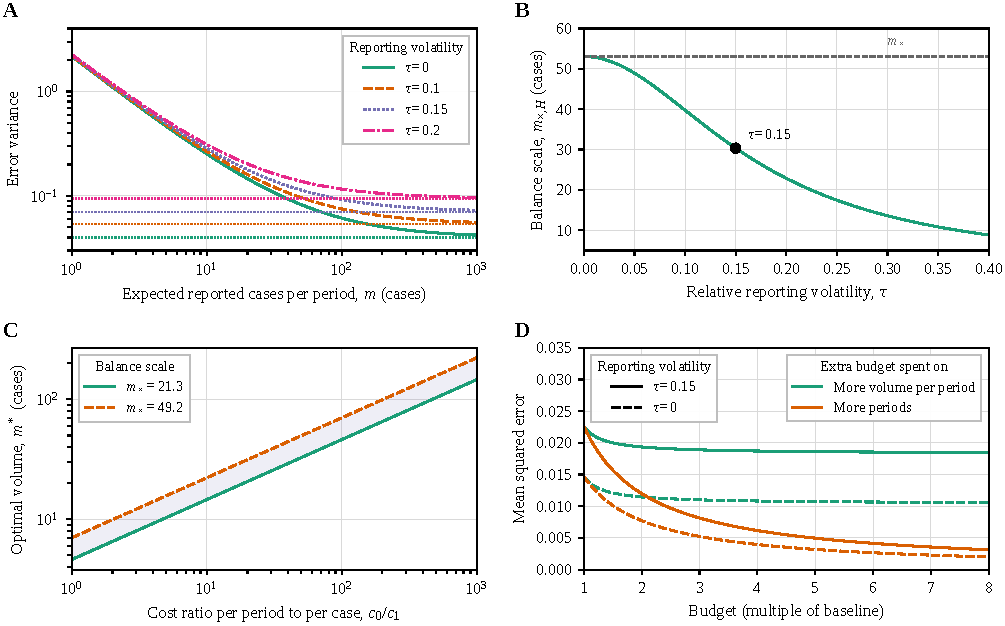
\includegraphics[width=0.92\linewidth]{figures/fig_02_heterogeneity_budget.pdf}
  \caption{Reporting heterogeneity and the allocation of a fixed surveillance budget. (A) Error variance against expected reported cases per period for four levels of relative reporting volatility; dotted lines mark the corresponding limits as case volume grows, set by environmental plus reporting variance. (B) Generalised balance scale against relative reporting volatility; the dashed line is the balance scale without reporting volatility, and the dot marks the volatility used in panel D. (C) Optimal number of reported cases per period against the price ratio $c_0/c_1$, for the two ends of the uncorrected scenario range of the balance scale, 21.3 and 49.2 cases per generation (labelled $m_\times$ in the panel); the band spans the range between them. (D) Mean squared error of the estimator of the mean reproduction number against total budget, when additional budget buys either more cases per period or more periods, with autocorrelated environmental and reporting variation, under baseline (solid) and standardised (dashed) reporting.}
  \label{fig:budget}
\end{figure}

A relative reporting volatility of $\tau=0.15$ added $v_H=0.0307$ to the limiting variance and reduced the balance scale from 53.1 to 30.4 cases (Fig.~\ref{fig:budget}A, B). The scenario parameters for influenza admissions give uncorrected balance scales of 21.3 to 49.2 cases per generation (Section~\ref{sec:meth-loss}); Section~\ref{sec:res-empirical} reports the latent value implied by the data. Over this range, the optimal case volume $m^*$ of Eq.~(\ref{eq:optimal-m}) was 14.6 to 22.2 cases per period for $c_0/c_1=10$ and 46.2 to 70.1 cases for $c_0/c_1=100$ (Fig.~\ref{fig:budget}C). In a hypothetical example with ten periods of 50 cases, autocorrelated environment ($\phi=0.5$) and reporting (with relative reporting perturbation autocorrelation $\psi=0.5$, see Appendix~\ref{app:random-denominator}) and $\tau=0.15$, the mean squared error of the mean was $22.57\times10^{-3}$, of which $10.40\times10^{-3}$ was environmental, $7.88\times10^{-3}$ reporting and $4.29\times10^{-3}$ sampling (Table~\ref{tab:s7}). A tenfold increase in case volume reduced it to $18.71\times10^{-3}$, whereas standardising reporting reduced it to $14.65\times10^{-3}$ and four times as many periods to $6.17\times10^{-3}$. At twice the baseline budget, spending the increment on cases gave $19.35\times10^{-3}$ and spending it on periods gave $11.98\times10^{-3}$ (Fig.~\ref{fig:budget}D).

\subsection{Calibration of apparent weekly statistics by simulation}
\label{sec:res-sim}

\begin{figure}[t]
  \centering
  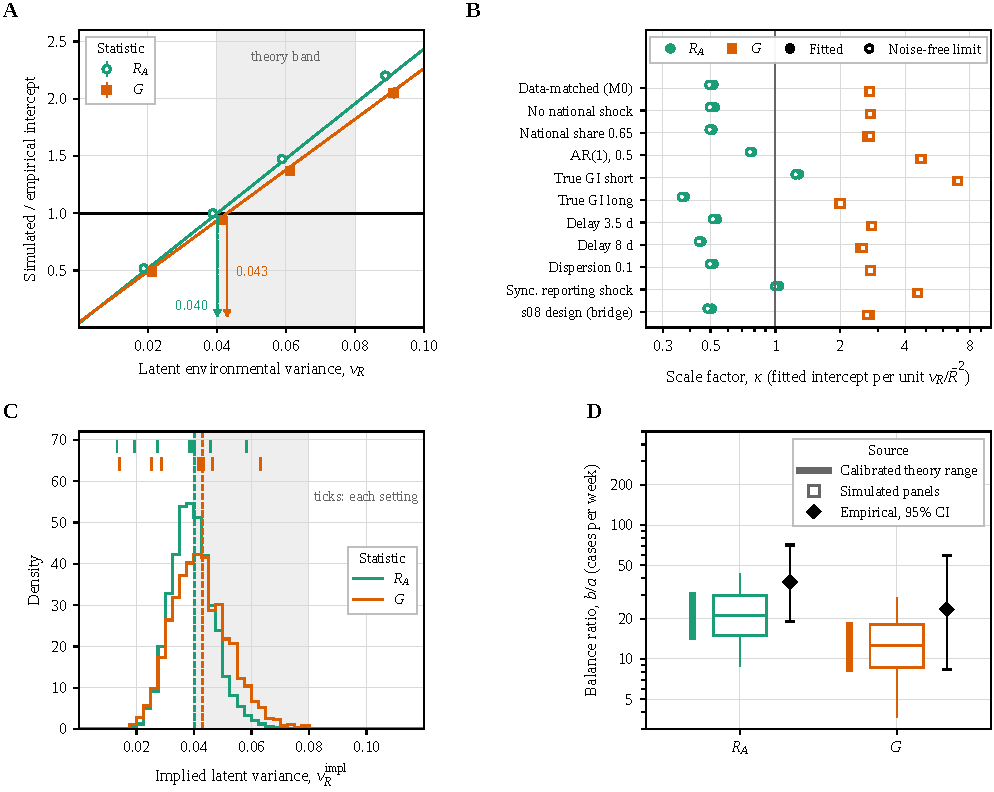
\includegraphics[width=\linewidth]{figures/fig_03_sim_inversion.pdf}
  \caption{Simulation-based inversion from apparent statistics to latent dynamics. (A) Calibration lines from 200 simulated panels per cell that reproduce the observed seasons, window lengths, state sizes, national week shocks and reporting delay. Fitted intercepts are scaled by the empirical intercept. Dashed drop lines mark where each line meets the data, giving the implied latent variance $v_R$. (B) Scale factor $\kappa$ linking the fitted intercept to $v_R/\Rbar^2$ for each simulation setting. Filled markers are fitted values and open markers the noise-free limit. (C) Distribution of the implied $v_R$ under the data-matched setting. Uncertainty combines the two-way bootstrap of the data with Monte Carlo error of the calibration. Top ticks show the point values of the other settings. (D) Simulated per-panel $b/a$ and the calibrated theoretical range, against empirical estimates with 95\% intervals. Grey bands mark $v_R=0.04$--0.08.}
  \label{fig:inversion}
\end{figure}

The empirical statistics are apparent quantities. The weighted growth ratio $G$ compounds more than one generation of growth into a week, and the renewal-type ratio $R_A$ maps weekly growth back to the generation scale through an assumed generation interval (Section~\ref{sec:meth-stats}). Their intercepts therefore need a calibration before they can be compared with $v_R$. We built this calibration in a simulation that reproduces the observed panel (Section~\ref{sec:meth-inversion}). It keeps the four seasons, the rule-window lengths and the initial admissions of each state, and adds a national week shock that carries 45\% of $v_R$ and the delay from infection to admission. We simulated 200 panels at each of four values of $v_R$. The mean fitted intercept rose linearly with $v_R$ for both statistics (Fig.~\ref{fig:inversion}A), and no cell mean departed from the fitted line by more than 0.60 Monte Carlo standard errors.

Expressed as a scale factor on $v_R/\Rbar^2$, the fitted intercept was $\kappa=0.516$ for $R_A$ and 2.729 for $G$, close to the noise-free limits of 0.493 and 2.745 (Fig.~\ref{fig:inversion}B). A simpler design with 500 independent states and six observation weeks gave noise-free limits of 0.485 and 2.698, in line with the medians of 0.484 and 2.68 over the 17 scenarios of the first simulation. The data-matched panels also reproduced the dependence structure of the data. The intraclass correlation of weekly losses within calendar weeks was 0.258 for $R_A$ and 0.310 for $G$ in simulation, against 0.253 and 0.310 in the data, and the national-week share of the simulated $R_A$ intercept was 0.43, against 0.41 observed. Across settings that changed one ingredient at a time, $\kappa$ for $R_A$ moved most with the true generation interval (1.287 for a mean of 2.2 days and 0.380 for 4.3 days, with the statistic still computed at 3.6 days), with autocorrelation of transmission between weeks (0.780 at $\phi=0.5$) and with a synchronous shock to reported counts (1.041). It changed little with the national share of the shock, the admission delay or the offspring dispersion (0.454 to 0.535; Table~\ref{tab:s8}).

\subsection{Empirical intercepts and the implied environmental variance}
\label{sec:res-empirical}

\begin{figure}[t]
  \centering
  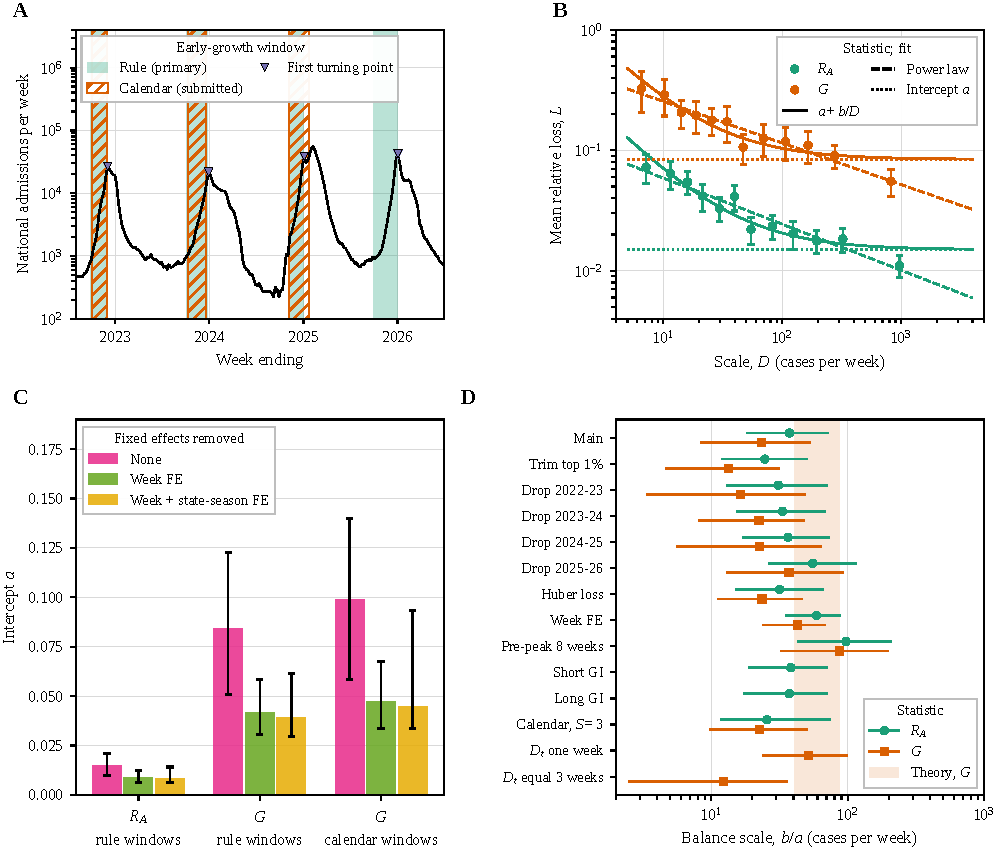
\includegraphics[width=0.86\linewidth]{figures/fig_04_empirical_loss.pdf}
  \caption{Relative loss of two apparent weekly statistics in influenza hospital admissions. (A) National weekly admissions on a logarithmic scale; shading marks the rule-based early-growth windows of the primary analysis, hatching marks the calendar windows of the earlier analysis, and triangles mark the first national turning point of each season. (B) Binned mean relative loss against reporting scale for the renewal-type ratio and the weighted growth ratio, with the fitted affine curve, a power law without intercept used for comparison and the fitted intercept; bin error bars ignore clustering. (C) Intercept before adjustment, after removing national-week effects and after also removing state-season effects, with two-way bootstrap intervals. (D) Ratio of slope to intercept under sensitivity variants; the band is the uncalibrated theoretical range for the growth ratio with the denominator correction, and Fig.~\ref{fig:inversion}D gives the calibrated range.}
  \label{fig:floor}
\end{figure}

In the rule-defined early-growth windows of four seasons, 1748 state-weeks in 42 calendar weeks gave a renewal-type ratio intercept of $a=0.0150$ (95\% CI 0.0100 to 0.0208), slope $b=0.560$ (95\% CI 0.367 to 0.769) and $b/a=37.4$ (95\% CI 19.1 to 71.0) (Fig.~\ref{fig:floor}B; Table~\ref{tab:s1}). The weighted growth ratio in the same windows gave $a=0.0840$ (95\% CI 0.0498 to 0.1248) and $b/a=23.5$ (95\% CI 8.4 to 59.7) from 1756 state-weeks. The eight additional state-weeks have a reporting scale $D_t$ of at least five but fewer than five admissions in the current week, which $R_A$ requires because its scale is the single-week count. In the three calendar windows of the earlier analysis, the growth ratio gave $a=0.0991$ (95\% CI 0.0569 to 0.1382) and $b/a=22.6$ (95\% CI 9.0 to 52.2). Within the affine model, all bootstrap replicates gave a positive intercept for both rule-window specifications, as did 99.95\% for the calendar windows. The bootstrap standard deviation of $a$ was 1.95 to 4.68 times that obtained by resampling states only.

The ratio $b/a$ varied across specifications by a factor of 3.9 for $R_A$, from 24.7 after trimming the most influential 1\% of losses to 97.1 in peak weeks, and by a factor of 7.1 for $G$, from 12.2 with equal denominator weights to 86.8 in peak weeks (Fig.~\ref{fig:floor}D). Generation interval variants changed it by less than 3\% for $R_A$. Over the observed range of scales, a power law without an intercept fitted the binned losses about as well as the affine form (bootstrap $p=0.114$ for $R_A$, 0.438 and 0.418 for $G$; Table~\ref{tab:s2}). Cross-validation by state and by season did not consistently favour the affine form, and a power analysis found no fraction of the estimated intercept detectable with 80\% power (Table~\ref{tab:s2}). The data therefore do not distinguish a positive floor from a loss that keeps declining as a power of the reporting scale. The affine form was retained because its parameters correspond to Proposition~\ref{prop:average} and enter the calibration directly. Under the power law no balance scale exists, so the intercept, the apparent balance ratio and the quantities derived from them below are conditional on the affine form.

Mapping each empirical intercept through its calibration line gave an implied latent variance of $v_R^{\mathrm{impl}}=0.040$ (95\% CI 0.026 to 0.056) for $R_A$ and 0.043 (95\% CI 0.025 to 0.064) for $G$ (Fig.~\ref{fig:inversion}A, C). Bootstrap variation in the empirical intercept accounted for nearly all of this width, since the interval from calibration error alone was 0.0397 to 0.0406 for $R_A$. The scale factors of the two statistics differ by a factor of 5.3. Their implied variances differed by $-0.003$ (95\% CI $-0.012$ to 0.005), a ratio of 0.93 (95\% CI 0.78 to 1.18). The 90\% interval of this ratio, 0.81 to 1.13, lies within 0.80 to 1.25, so two one-sided tests at the 5\% level declare the two estimates equivalent within a margin of 20\%. This concordance serves as a model-consistency check under the reference simulator, although it has limited discriminating power across the wider sensitivity space where the two statistics also produced overlapping intervals in nine of the ten simulated settings (Table~\ref{tab:s8}). Both point values lie at the lower edge of the band of 0.04 to 0.08 used in the scenario calculations, and both intervals extend below it. On the latent scale, Proposition~\ref{prop:average} at the simulator values ($\Rbar=1.18$, $\rho=\rho_h=0.01$, $k=0.35$) gives a balance scale of 30.3 admissions per generation (95\% CI 21.7 to 46.3) for $R_A$, or about 59 per week at 1.94 generations per week. The apparent ratio of 37.4 is defined on the scale of $R_A$ and does not estimate this latent quantity directly. The latent scale moves with the implied variance; at the value of 0.026 obtained with a true mean generation interval of 2.9 days (below), the same formula gives about 47 admissions per generation, or roughly 110 per week.

Across ten settings, $v_R^{\mathrm{impl}}$ ranged from 0.013 to 0.063 (Fig.~\ref{fig:inversion}C; Table~\ref{tab:s8}). The true generation interval had the largest effect, giving 0.013 and 0.014 when it was shorter than the 3.6 days assumed by the statistic and 0.058 and 0.063 when it was longer. The interval of the primary estimate does not include this source of variation. The 95\% interval of the difference between the two statistics contained zero in nine of the ten settings; this non-rejection is the sense of agreement used in Table~\ref{tab:s8}. The exception replaced the transmission shock by a synchronous multiplicative shock to reported counts, which gave 0.019 for $R_A$ and 0.029 for $G$ (ratio 0.67; 95\% CI 0.39 to 0.90).

Three classes of sensitivity analyses examined the assumptions of the inversion (Table~\ref{tab:s10}). The lag-1 autocorrelation of deviations from state-season means was $-0.095$ (95\% CI $-0.168$ to $-0.019$) for $R_A$ and 0.123 (95\% CI 0.039 to 0.201) for $G$. Both statistics are autocorrelated by construction even when weekly shocks are independent; simulated panels with independent shocks gave means of $-0.074$ and 0.114, which placed the data at the 31st and 62nd percentiles. With a first-order coefficient of 0.25 the data fell at the 3rd and 10th percentiles, and with 0.5 below all simulated panels. The mean household serial interval of seasonal influenza has been estimated at 3.6 days (95\% CI 2.9 to 4.3) \citep{cowling2009estimation}, and direct estimates of the mean generation interval lie near the lower end of this interval \citep{chan2025estimating}. With a true mean generation interval of 2.9 days, the implied variance was 0.026 (95\% CI 0.017 to 0.036) for $R_A$ and 0.027 (95\% CI 0.016 to 0.040) for $G$; with 4.3 days it was 0.058 and 0.063. The autocorrelation of the data sat at the 2.5th and 9th percentiles of panels simulated with 2.9 days and at the 80th and 92nd percentiles with 4.3 days. This state-level check therefore does not favour the shorter interval, although it leaves the series of national-week means untested (Section~\ref{sec:meth-inversion}). The shorter interval did reproduce the empirical $b/a$. At $v_R=0.02$, the simulated value nearest its implied variance, the data sat at the 52.5th and 58th percentiles of the simulated $b/a$. Overdispersed weekly admissions with a variance-to-mean ratio of 1.5 or 2.0 kept the implied variance between 0.039 and 0.045. They raised the simulated $b/a$ at $v_R=0.04$ from 28.0 to 68.0 and 81.0 for $R_A$, and from 16.2 to 40.2 and 48.4 for $G$. These settings also gave lag-1 autocorrelations below the data for both statistics, so the data were more compatible with overdispersion smaller than a variance-to-mean ratio of 1.5 under this simulator.

On the scale of each statistic, the calibrated theory gave $b/a$ of 13.9 to 31.1 for $R_A$ and 8.0 to 18.8 for $G$ over eight combinations of $v_R\in\{0.04,0.08\}$, $k\in\{0.2,0.5\}$ and admission probability $\rho_h\in\{0.0056,0.021\}$ (Fig.~\ref{fig:inversion}D). The empirical point estimates of 37.4 and 23.5 lie above these ranges, and their 95\% intervals overlap them. Ratios from single simulated panels varied widely; 95\% of them lay between 8.8 and 42.7 for $R_A$ and between 3.6 and 28.6 for $G$, and the empirical values fall at the 93rd and 91st percentiles of these distributions. Overdispersed admissions and a shorter generation interval can each raise the simulated ratio to the empirical values (Table~\ref{tab:s10}). A further explanation lies outside the simulator, which gives every state the same intercept. If larger states average environmental variation over more local epidemics (Eq.~(\ref{eq:pooling})), part of the cross-sectional slope reflects spatial aggregation and the empirical $b/a$ is inflated.

\subsection{Multiscale decomposition of surveillance uncertainty}
\label{sec:res-multiscale}

The intercept contains a component shared by all states in a calendar week and a component specific to states (Fig.~\ref{fig:floor}C; Table~\ref{tab:s2}). Removing national-week effects reduced $a$ by 41\% (95\% CI 12 to 59) for $R_A$ and by 51\% (95\% CI 21 to 67) for $G$ in rule windows, and by 52\% for $G$ in calendar windows. Removing state-season effects as well changed the intercept little; for $R_A$ it was 0.0083 (95\% CI 0.0064 to 0.0141) after both adjustments, and the interval for the state-season component included zero in every specification. The intraclass correlation of the loss within calendar weeks was 0.253 for $R_A$ and 0.310 for $G$. The bootstrap reflected the same structure. Resampling weeks alone gave a standard deviation of $\hat{a}$ of 0.0021 for $R_A$ and 0.0158 for $G$, 1.46 and 1.87 times the values from resampling states alone, and two-way resampling gave 0.0028 and 0.0193.

The national-week component enters the loss of every state in the same week. More admissions in one state reduce only that state's count term, and averaging over states reduces only the state-specific term, so neither removes the shared component; only further weeks average it out. Pooling the mean weekly deviation over $J$ randomly chosen states reduced its variance to 0.39, 0.31 and 0.25 of the single-state value for $R_A$ at $J=5$, 10 and 51, and to 0.43, 0.36 and 0.31 for $G$ (Fig.~\ref{fig:design}C). These values approach the national-week component, which is 0.23 of single-state variance for $R_A$ and 0.29 for $G$, and come within 10\% of it at $J=33$ and $J=25$ respectively, as Eq.~(\ref{eq:pooling}) predicts for partly synchronised variation.

\subsection{Mandatory and voluntary reporting regimes}
\label{sec:res-reporting}

\begin{figure}[t]
  \centering
  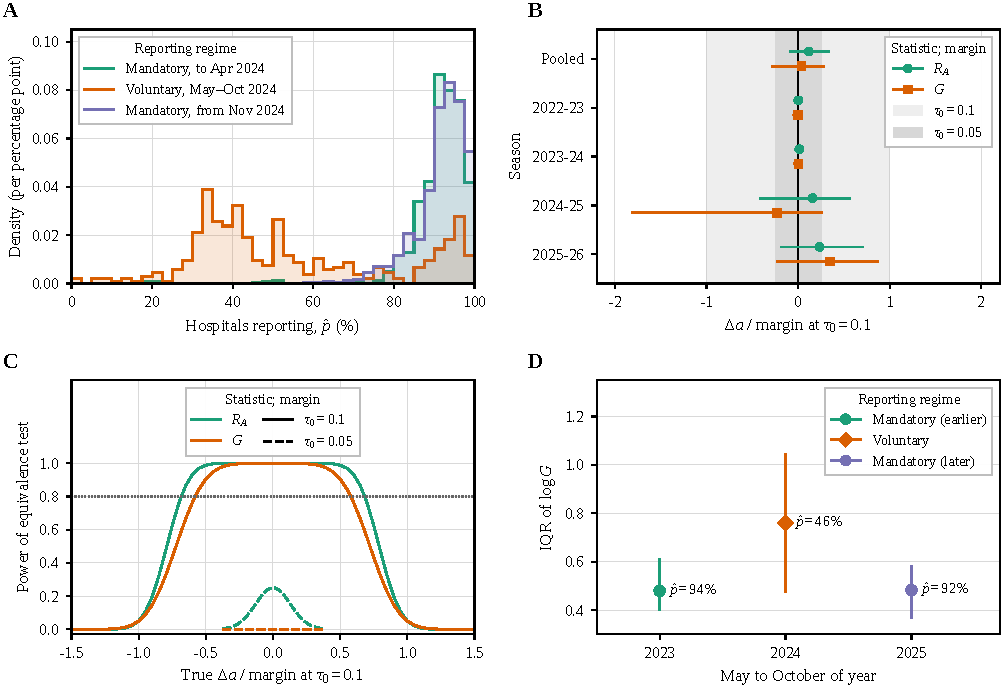
\includegraphics[width=0.86\linewidth]{figures/fig_05_reporting.pdf}
  \caption{Reporting completeness and the empirical intercept. (A) Distribution of the share of hospitals reporting influenza admissions under the three reporting regimes. (B) Change in the intercept when the statistic is adjusted for reporting coverage, pooled and by season, with 90\% paired bootstrap intervals. Each statistic is expressed relative to its own equivalence margin, and shaded bands show the margins implied by two thresholds of reporting volatility. (C) Power of the two one-sided equivalence test against the true change, for both statistics and both margins, with a conventional power reference. (D) Interquartile range of the logarithm of the growth ratio over May to October in three calendar years; the year with voluntary reporting is highlighted, and labels give median reporting completeness.}
  \label{fig:reporting}
\end{figure}

Among state-weeks with a reporting scale of at least five, the median share of hospitals reporting was 92.3\% in the first mandatory period, 45.7\% under voluntary reporting and 92.9\% after mandatory reporting resumed (Fig.~\ref{fig:reporting}A). In the rule windows the median was 93.7\%, and 79.8\% of state-weeks had at least 90\% of hospitals reporting. Within these windows, adjusting each statistic for the reporting share changed the intercept of $R_A$ by $\Delta a=0.29\times10^{-3}$ (90\% CI $-0.22\times10^{-3}$ to $0.85\times10^{-3}$) and that of $G$ by $0.37\times10^{-3}$ (90\% CI $-2.83\times10^{-3}$ to $2.81\times10^{-3}$) (Fig.~\ref{fig:reporting}B; Table~\ref{tab:s3}). Both changes were equivalent to zero within margins set at a relative reporting volatility of $\tau_0=0.10$. These margins equal 17\% (95\% CI 12 to 25) of the intercept of $R_A$ and 12\% (95\% CI 8 to 20) of that of $G$, and they depend on the sample mean of each statistic through Eq.~(\ref{eq:tost}). The measured change was 2.0\% of the intercept for $R_A$ (95\% CI $-2.4$ to 6.1; one-sided 95\% upper bound 5.3\%, the 95th percentile of the bootstrap distribution of the share) and 0.4\% for $G$ (95\% CI $-4.4$ to 4.0; upper bound 3.5\%), and all four seasons for $R_A$ and three of four for $G$ were equivalent individually. At $\tau_0=0.05$, with margins of about 4\% and 3\% of the intercepts, neither change was equivalent, and the power of the test at a true change of zero was 0.25 for $R_A$ and 0 for $G$ (Fig.~\ref{fig:reporting}C). Because most state-weeks in the windows had nearly complete participation, these tests bound the effect of small departures from full participation and do not extend to low participation.

The voluntary period gave the only contrast in which reporting completeness was low. Over May to October, the interquartile range of $\log G$ was 0.759 in 2024 under voluntary reporting, against 0.479 in 2023 and 0.483 in 2025 (Fig.~\ref{fig:reporting}D; Table~\ref{tab:s4}). The ratio of 2024 to 2023 was 1.58 (95\% CI 0.95 to 2.23) and that of 2024 to 2025 was 1.57 (95\% CI 0.95 to 2.39), whereas the placebo ratio of 2025 to 2023 was 1.01 (95\% CI 0.72 to 1.25). Median reporting scales in these months were similar (15.6, 16.6 and 16.2 admissions), and matching state-weeks on reporting scale gave ratios of 1.68 and 1.58. Matching on calendar month gave a median ratio of 1.33, with the ratio above one in nine of twelve month-by-year comparisons. COVID-19 admissions showed ratios of 1.62 against 2023 and 1.18 against 2025, and RSV admissions a ratio of 1.36 against 2025. All of these comparisons use the same off-season of 2024 and are not independent replications. In 44 states with laboratory data, laboratory $R_A$ correlated with hospital $R_A$ at $r=0.31$ and shared 0.230 (95\% CI 0.043 to 0.418) of the hospital intercept.

\subsection{Diminishing returns and surveillance design}
\label{sec:res-design}

\begin{figure}[t]
  \centering
  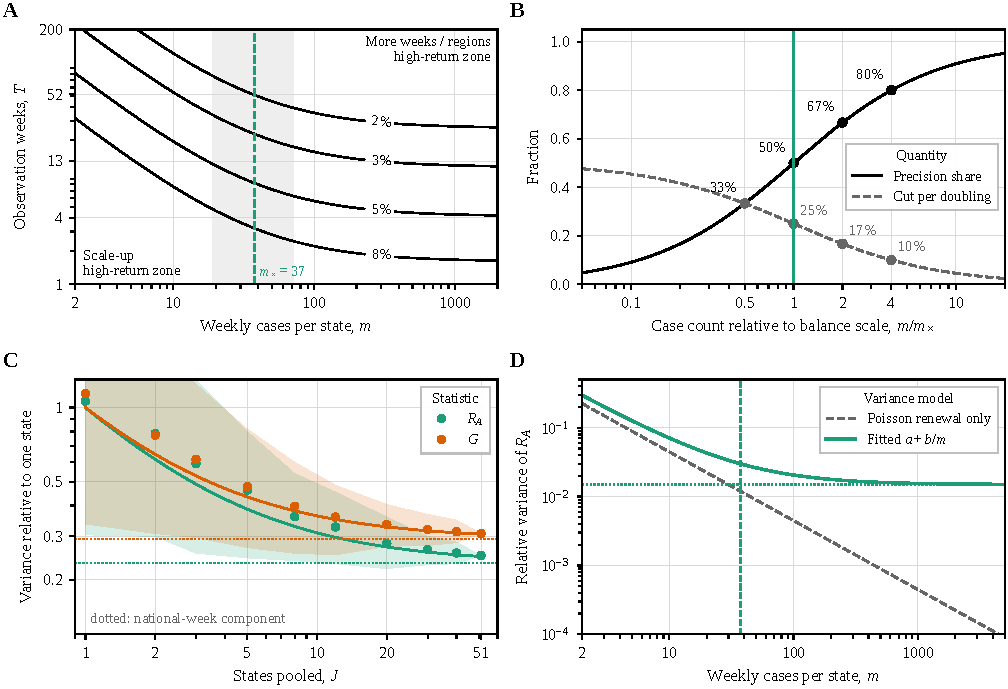
\includegraphics[width=\linewidth]{figures/fig_06_design_nomogram.pdf}
  \caption{Surveillance design nomogram. (A) Observation weeks needed for the relative standard error of a single state's mean renewal ratio $R_A$ to reach 2--8\%, by weekly admissions $m$, on the scale of the statistic and ignoring autocorrelation within states. The dashed line marks the apparent balance ratio $b/a$ of $R_A$ (labelled $m_\times$ in the legacy panel asset), and the grey band its 95\% interval. To its left, added cases give most of the gain. To its right, contours flatten and added weeks or regions give most of the gain. (B) Share of attainable precision, $m/(m+\mx)$, and the variance reduction from one doubling of $m$. (C) Variance of the mean weekly deviation pooled over $J$ states, relative to one state, for $R_A$ and the growth ratio $G$. Points and bands come from random state subsets; dotted lines show the national-week component. (D) Relative variance of $R_A$ under the Poisson renewal variance alone and under the fitted $a+b/m$.}
  \label{fig:design}
\end{figure}

Under $V(m)=a+b/m$, the share of the precision attainable at unlimited case volume is $m/(m+\mx)$, and one doubling of $m$ reduces variance by the fraction $\mx/[2(m+\mx)]$ (Proposition~\ref{prop:average}). The share is 33\%, 50\%, 67\% and 80\% at $m=0.5$, 1, 2 and 4 times $\mx$, a doubling from these points cuts variance by 33\%, 25\%, 17\% and 10\%, and 90\% of attainable precision requires $m=9\mx$ (Fig.~\ref{fig:design}B). With the apparent balance ratios of 37.4 for $R_A$ and 23.5 for $G$, 55\% and 65\% of state-weeks in the rule windows lay above the ratio of the corresponding statistic. These shares refer to the apparent scale. The latent balance scale implied by the data, about 59 admissions per week (Section~\ref{sec:res-empirical}), is higher, so fewer state-weeks (approximately 43.5\%) lie above it on the latent per-generation scale, and a shorter generation interval would raise the latent scale further (roughly 110 per week at 2.9 days). For a single state, the number of observation weeks needed to reach a given relative standard error of mean $R_A$ fell steeply with admissions below $\mx$ and changed little above about $4\mx$ (Fig.~\ref{fig:design}A). Substituting the empirical apparent balance ratio $b/a$ into the allocation formula gives apparent-scale design analogues of the optimal case volume: $m^*=19.4$ (95\% CI 13.8 to 26.6) for $R_A$ and 15.3 for $G$ at $c_0/c_1=10$, and $m^*=61.2$ and 48.4 at $c_0/c_1=100$. Note that at $c_0/c_1=100$, the economic switching threshold $m^*=61.2$ exceeds the apparent balance ratio $37.4$, confirming that the condition for prioritising additional periods over cases per period is $m > m^*$, whereas the balance scale itself governs the onset of diminishing marginal returns.

The fitted variance departs from that of a Poisson renewal model, in which the error variance of the estimate is $\Rbar/m$ and has no term that persists as $m$ grows (Fig.~\ref{fig:design}D). On the apparent scale of $R_A$, the fitted slope ($b=0.560$) was 1.25 times the delta-method Poisson renewal slope $b_P = 0.446$ (computed as $\E[\kappa_A^2(1+C_t/C_{t+1})]$, which propagates Poisson count variance through the nonlinear renewal transformation), and the fitted variance was twice the Poisson variance at $m=22$ and ten times at $m=261$. On the latent scale of Proposition~\ref{prop:average}, with $v_R=0.040$, the corresponding values were $m=28$ and $m=262$.

Seasons limit any estimate of variation between seasons (Fig.~\ref{fig:seasons}). Season-specific intercepts of $R_A$ were 0.0137, 0.0062, 0.0127 and 0.0225, with a random-effects mean of 0.0125 (95\% CI 0.0022 to 0.0227) and $I^2=0.47$ (Table~\ref{tab:s5}). For $G$ the random-effects mean was 0.0619 (95\% CI 0.0066 to 0.1171) in rule windows and 0.0735 (95\% CI $-0.0558$ to 0.2028) in calendar windows. The relative standard error of any unbiased estimate of the between-season variance is at least 1.00 with three seasons and 0.82 with four (Corollary~\ref{cor:season}). Intercept ratios for alternative denominator weights showed $q_1<1<q_2$ for influenza, COVID-19 and RSV, for example $q_1=0.688$ and $q_2=1.539$ for influenza in calendar windows (Table~\ref{tab:s6}). Epidemic growth with reporting noise and no environmental variation gave ranges of 0.63 to 0.89 for $q_1$ and 1.13 to 1.58 for $q_2$ in calendar windows, so this ordering does not discriminate between mechanisms. Of 40 one-sided tests, 21 were significant before correction, 18 after Benjamini--Hochberg correction and 10 after Holm correction, all of them for influenza and none for departures from the null ranges.
